\section{User-configurable Event Scheduling}
\label{sec:using event scheduler}
This section describes a feature for scheduling of arbitrary deterministic and
stochastic events during experiment execution.

\subsection{Principle of operation}
The control plane in IMUNES is extended to retain control over the experiment
execution after initial topology instantiation, allowing for user-scheduled
events to influence selected parameters during run time.

The current implementation allows for the event scheduler to assume control
over selected link properties such as:
\begin{itemize}
\item bandwidth
\item delay
\item bit error rate
\item packet duplication
\item visual attributes
\begin{itemize}
\item line width
\item line color
\end{itemize}
\end{itemize}

The event scheduler supports two general classes of schedulable events:
one-time changes and periodic functions. 

One-time events update the selected parameter at requested point in time,
leaving that parameter constant throughout rest of the experiment execution, or
until another event updates it to a new value at some later point in time. 

Periodic functions allow for time-variant functions to be applied to selected
parameters by specifying those functions as single events. Subsequently
scheduled events acting upon the same parameter will cancel the current
periodic function and replace it with either a constant value or another
periodic function.

\subsection{Configuring events with events editor}
Events can be specified in the \emph{Events editor} (Figure
\ref{fig:event_editor}). To open the \emph{Events editor} select the
\emph{Events} $\to$ \emph{Events editor} option. The editor is divided into two
elements. The left side element contains a list of all links. The right side
element contains events configured on the selected link. This dialog allows you
to edit events on that link. To save the event scheduling configuration you
need to click on \emph{Apply} button. The events editor gives you the
possibility to start or stop the event scheduling during experiment execution.
This can be also done from the \emph{Events} menu in the menubar.

\begin{figure}[H]
	\centering
	\vspace{10pt}
	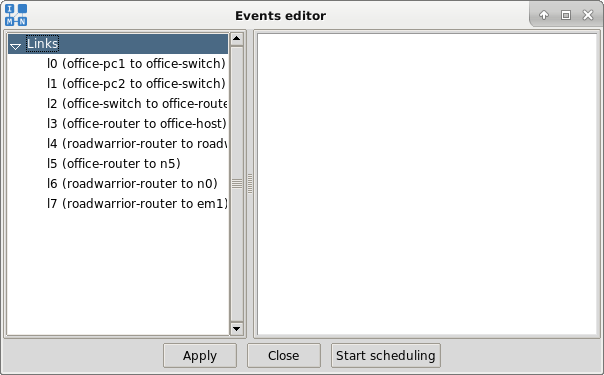
\includegraphics[width=0.65\textwidth]{./images/event_editor.png}
	\caption{\emph{Events editor}}
	\label{fig:event_editor}
\end{figure}

Each event entry occupies a single line of text, consisting of four fields:
deadline, target parameter, function and function parameters. The first field,
deadline, is specified as an integer number of seconds since experiment
instantiation. The second field, target parameter, may be one of the following:
bandwidth, delay, ber, duplicate, width or color. The remainder of the line is
further parsed as a function. The type of the function is determined by the
leading keyword, which may be either const, ramp, rand or square. When saving
the configuration through the events editor a syntax check will be performed.
If the syntax is wrong the configuration will not be saved and a popup dialog
will show the first line that has a syntax error.

\subsubsection{Const}
The const function accepts one parameter, the target value. After the deadline
time the parameter will constantly be equal to the target value.

\subsubsection{Ramp}
Behavior of the ramp function is determined by three arguments: initial value,
delta, and period, which are all integers. The first argument represents the
initial function value. The second is the delta value, which may be both
positive or negative, which is added to the previous value of the function at
each period. The third argument is the period, determining how often will the
delta value be added to the current function value.

\subsubsection{Rand}
The rand function is determined by three arguments: lower bound, upper bound,
and period; all of which are integers. The function will assume a random value
between lower and upper bound after each period (in seconds) expires.

\subsubsection{Square}
Finally, the square function has three arguments as well: low value, high
value, and period; all integer numbers. The resulting function will flip from
low value to high and vice versa after each period (in second) expires.

\subsubsection{Example}
The following example illustrates a possible event scheduling scenario that can be entered in the Event editor window (Figure \ref{fig:event_editor}):

\begin{alltt}
    30 bandwidth ramp 128000 8000 2
    30 delay rand 80000 120000 8
    60 delay square 100000 200000 10
    60 ber const 1
    90 ber const 0
    120 delay const 0
\end{alltt}

At t = 30 s, bandwidth of the selected link will be set to 128 Kbps, and will
continue to grow at a rate of 8 Kbps each 2 s.

Also at t = 30 s, the delay will begin assuming a random value between 80 ms
and 120 ms, and will continue to change the setting to new random values in the
same range each 8 s.

At t = 60 s, the delay will cease to assume random values, and instead it will
begin to oscillate between two discrete values, 100 ms and 200ms, each 10 s.

Also at t = 60 s, the bit error rate (BER) will be set to 1, resulting in all
frames traversing the link to be silently dropped.

At t = 90 s, the BER is reset back to 0, allowing for all frames to traverse
the link without artificial losses.

At t = 120 s, the oscillation of the delay parameter will stop, and delay will
be reset to 0 ms for the rest of the experiment execution time.

The current time is shown on the status bar after the zoom value. (Figure
\ref{fig:statusbar_execute})

\subsection{Configuring events through configuration file}
\textbf{NOTE:} It is advised to use the Events editor to configure event
scheduling because it includes a syntax check. In the case of configuring
events through configuration file, the wrong syntax will be silently ignored.

IMUNES experiments are defined via plain-text configuration files, which
currently describe virtual nodes and links, as well as additional objects
related only to GUI visual properties and annotations. The other way to
configure events is manual editing of an existing configuration file.

The example bellow shows a configuration section describing a virtual link in
an IMUNES experiment. The link l0 connects virtual nodes n0 and n1, has the
bandwidth constraint set to 128 Kbps, and has the thickness of the line
representing the link in the GUI set to 6 pixels. All of the mentioned
properties are directly controllable via the IMUNES GUI. The configuration for
link l0 also includes an empty placeholder for schedulable events, meaning that
no events have been programmed for this link.

\begin{alltt}
link l0 \{
    width 6
    nodes \{n0 n1\}
    bandwidth 128000
    \emph{events \{}
    \emph{\}}
\}
\end{alltt}

The events section in the configuration file accepts the same commands as does
the Events editor in the GUI.

